\begin{refsection}
    \renewcommand{\thefigure}{\arabic{figure}}
    
    \chapterTwoLines
    {O material dourado como recurso didático no ensino do algoritmo da subtração}
    {Uma experiência em sala de aula}
    \label{chap:material-dourado}

    \begin{otherlanguage}{english}

    \fakeChapterTwoLines
    {The golden material as a didactic resource in the subtraction algorithm teaching}
    {A classroom experience}

    \end{otherlanguage}
    
    \articleAuthor
    {Verônica Umbelino Souza de Carvalho}
    {\textit{Minicurrículo e contato não disponibilizados pela autora.}}
    
    \articleAuthor
    {Anilda Pereira da Silva Guimarães}
    {Graduada em Ciências com habilitação em Matemática pela Universidade Federal do Rio Grande do Norte (1981). Graduada em Pedagogia pela Universidade Federal do Rio Grande do Norte (1987). Mestra em Educação pela Universidade Federal do Rio Grande do Norte (2005). Atualmente é professora do Instituto de Educação Superior Presidente Kennedy. ID Lattes: 9681.3290.9483.0259.}
    
    \begin{galoResumo}
        \marginpar{
            \begin{flushleft}
            \tiny \sffamily
            Como referenciar?\\\fullcite{SelfCarvalhoAndGuimarães2021material}\mybibexclude{SelfCarvalhoAndGuimarães2021material}, p. \pageref{chap:material-dourado}--\pageref{chap:material-douradoend}, \journalPubDate{}
            \end{flushleft}
        }
        A questão que norteia este estudo é uma experiência realizada com a utilização do Material Dourado como facilitador da compreensão da subtração com reserva, numa turma do 4º ano do Ensino Fundamental de uma escola estadual localizada no município de Santa Cruz/RN. Esse trabalho foi motivado por tanto presenciar nas reuniões pedagógicas, a angústia de alguns professores relatando as dificuldades que seus alunos apresentam para compreender o algoritmo da subtração, em especial, a subtração com reserva. A pesquisa foi desenvolvida com base na pesquisa ação, onde buscamos aplicar algumas atividades de intervenção didática. O referencial teórico em que se baseou esse estudo aborda a importância dos materiais manipuláveis, em particular o Material Dourado, para uma melhor compreensão nos aspectos ensino/aprendizagem da Matemática. Assim, recorremos a \textcite{NACARATO2005trabalho}, \textcite{BERTONAndITACARAMBI2009Números}, \textcite{LORENZATO2006Começar}, \textcite{CENTURIÓN1995Números}, dentre outros, por reconhecerem a importância do uso do material concreto como um recurso didático facilitador no processo de ensino e aprendizagem. Podemos concluir que o uso do Material Dourado no ensino da matemática, além de facilitar a compreensão do desagrupamento na subtração, dá às relações numéricas abstratas uma imagem mais concreta, facilitando a compreensão, o desenvolvimento do raciocínio lógico, tornando o aprendizado bem mais agradável, pois é dada ao aluno a oportunidade de construir seus conhecimentos de uma forma mais interativa, dinâmica e prazerosa.
    \end{galoResumo}
    
    \galoPalavrasChave{Material Dourado. Algoritmo da subtração. Aprendizagem.}
    
    \begin{otherlanguage}{english}

    \begin{galoResumo}[Abstract]
        The issue that guides this paper is an experience carried out with the use of the golden material as a facilitator to understand the subtraction with reserve in a 4th grade classroom from the elementary school in a public state school located in Santa Cruz/RN region. This paper has been motivated after attending during pedagogical meeting the anguish of some teachers who reported the difficulties their students had in order to understand the subtraction algorithm. In particular, the subtraction with reserve. The research was developed based on the action research, where we sought to apply some didactic intervention activities. The theoretical reference in which this paper was based on approaches the importance of manipulable materials, in particular, the golden material, for a better comprehension related to the teaching learning of mathematics. Thus, we had as support \textcite{NACARATO2005trabalho}, \textcite{BERTONAndITACARAMBI2009Números}, \textcite{LORENZATO2006Começar}, \textcite{CENTURIÓN1995Números}, among others, since they recognize the importance of the use of a solid material as a didactic resource on the teaching and learning process. We can conclude that the use of the golden material in the mathematics teaching, in addition to make the comprehension/understanding of the subtraction ungrouping easier. By giving the abstracts numerical relation a more concrete image, facilitating the understanding, logical thinking development, making the learning enjoyable, since it gives the students the opportunity to build their knowledge in a more interactive, dynamic and enjoyable way. 
    \end{galoResumo}
    
    \galoPalavrasChave[Keywords]{Golden Material. Subtraction Algorithm. Learning.}
    \end{otherlanguage}

    \section{Introdução}

    A Matemática é uma disciplina que está presente em todos os níveis da educação, e é considerada pela maioria das instituições escolares a disciplina que causa o maior índice de reprovação e, consequentemente, o desinteresse por parte dos educandos por essa área do conhecimento. Para agravar ainda mais essa situação, a prática educativa no ensino da Matemática muitas vezes é realizada na sala de aula de forma abstrata e descontextualizada da realidade do educando, visto que geralmente o professor adota procedimentos, tais como: expor e/ou explicar o conteúdo; passar uma lista de exercícios; e fazer a correção destes. Sobre isso, Lorenzato afirma: Palavras não alcançam o mesmo efeito que conseguem os objetos ou imagens, estáticas ou em movimento. Palavras auxiliam, mas não são suficientes para ensinar. [\dots] o fazer é mais forte que o ver ou ouvir [\dots] \cite[p.~17--18]{LORENZATO2006Começar}. 

    Sabe-se que a Matemática se constitui em um saber que está presente nas ações do dia a dia, por isso uma inquietação/indagação motivou a pesquisa: por que um saber tão presente nas decisões do cotidiano é objeto de retenção na escola? Intervir nessa realidade de modo a encontrar novas formas de abordagem no processo ensino-aprendizagem da Matemática tornou-se um desafio. Certamente, são inúmeras as dificuldades encontradas no ensino e aprendizagem desta disciplina, mas aqui o objetivo consiste em analisar como o Material Dourado pode contribuir para a aprendizagem da subtração com reserva numa turma do 4º ano do Ensino Fundamental. 

    Os procedimentos metodológicos necessários à realização deste trabalho foram realizados na perspectiva da pesquisa ação, trabalhando a matemática de maneira construtiva e significativa através de uma sequência de atividades com o uso do Material Dourado. Esse material pode ser encontrado na maioria das escolas públicas do Brasil, porém, muitas vezes fica obsoleto em algum espaço escolar porque a maioria dos professores não sabe utilizá-lo, ou não acredita que o uso deste material, mediado pelo professor, possa contribuir significativamente para a aprendizagem. Os sujeitos desta pesquisa foram os alunos do 4º ano --- turno vespertino --- da Escola Estadual Isabel Oscarlina Marques, localizada no município de Santa Cruz/RN. 

    O referencial teórico que embasa esta pesquisa aponta a importância dos materiais manipuláveis, em particular o Material Dourado, para uma melhor compreensão dos conceitos matemáticos ligados às operações fundamentais e a sua relação no aspecto ensino/aprendizagem da Matemática. Assim, recorre-se a \textcite{NACARATO2005trabalho}, \textcite{BERTONAndITACARAMBI2009Números}, \textcite{CENTURIÓN1995Números} e \textcite{LORENZATO2006Começar}, entre outros. Busca-se através destes teóricos fundamentar a relevância de trabalhar com material concreto para o desenvolvimento do raciocínio lógico-matemático da criança.  

    Os problemas de aprendizagem da Matemática no Ensino Fundamental tratados neste trabalho dizem respeito aos fatores que contribuem para que a Matemática seja vista como uma disciplina cansativa e com maior índice de reprovação. Tornar suas aulas mais lúdicas, com atividades que disponibilizem o uso de materiais concretos, apresentando questões que partam da realidade do aluno foi a proposta utilizada nessa pesquisa para se chegar a um resultado mais satisfatório.  

    Entende-se que cabe ao educador por meio da intervenção pedagógica propiciar atividades que levem a uma aprendizagem significativa. Para que isso ocorra é necessário que o professor reflita sobre sua prática pedagógica, compreendendo o aluno como alguém que pode sentir prazer em aprender e não como um mero executor de tarefas.  

    Ensinar exige reflexões para que se contribua significativamente na formação de cidadãos que atendam as demandas do século XXI. Nessa perspectiva, desencadeou-se esse estudo, tendo como foco o uso do Material Dourado no ensejo de facilitar a aprendizagem da subtração com reserva através do uso desse material. 

    Para melhor compreensão, organiza-se este trabalho em cinco seções: A primeira, a introdução, onde situam-se o tema, o objetivo e a metodologia utilizada. A segunda seção traz um resgate teórico a respeito do uso do Material Dourado como recurso didático. A terceira discorre sobre o algoritmo da subtração. A quarta seção enfoca a experiência vivenciada na turma do 4º ano, relatando cada encontro realizado e, por fim, a quinta tece as considerações finais sobre a pesquisa realizada.

    \section{Material dourado: o que dizem alguns teóricos}

    \textcite{BERTONAndITACARAMBI2009Números} afirmam que Montessori criou o Material Dourado para trabalhar aritmética com as crianças que apresentavam distúrbios de aprendizagem. O nome dourado se deve à versão original que era feita com contas douradas. Quando foi industrializado, esse material passou a ser feito de madeira, mantendo o nome original. O material é constituído por cubinhos, barras, placas e o cubo, apresentando as regras de agrupamento na base 10. A manipulação e uso desse recurso podem ajudar na compreensão das operações fundamentais, reforçando a noção de troca no sistema posicional.  

    O Material Dourado propicia aos alunos descobrirem as relações entre as peças que o compõe, a saber: uma barra tem dez cubinhos, uma placa tem dez barras e o cubo tem dez placas. Isso é constituído para representar um sistema de agrupamento, associando o modelo didático com o conceito matemático. 

    No princípio, esse material foi criado com o intuito de auxiliar nas atividades que propiciassem o ensino e a aprendizagem do sistema de numeração decimal-posicional e, consequentemente, em métodos para efetuar as operações fundamentais. Hoje pode ser utilizado para o estudo de frações, conceituação e cálculo de áreas e volumes, trabalho com números decimais, raiz quadrada entre outros. Nesta pesquisa utilizou-se o Material Dourado para se trabalhar a subtração com reserva, objeto desse estudo. Atualmente, o material é apresentado conforme a Figura \ref{fig:material-dourado}.

    \begin{figure}[ht]%
        \centering%
        \caption{Material Dourado}%
        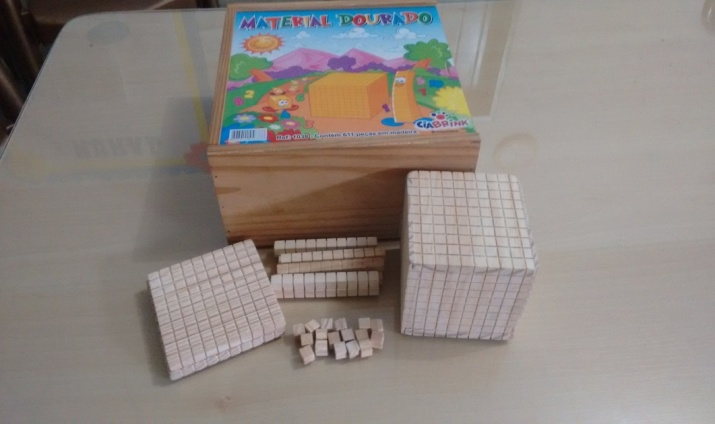
\includegraphics[width=.5\textwidth]{articles/05-material-dourado-com/figura1.jpeg}%
        \caption*{Fonte: Arquivo pessoal.}%
        \label{fig:material-dourado}%
    \end{figure}%

    O Material Dourado é um recurso didático riquíssimo, pois além de ser muito versátil ele tem como base ideológica primordial a educação sensorial da criança, a qual pode ser elencada, segundo \cite[p.~2]{DALTOÉAndStrelowTrabalhando} da seguinte forma:

    \begin{enumerate}
        \item desenvolve na criança a independência, a confiança em si mesma, a concentração, a coordenação e a ordem; 
        \item gera e desenvolve experiências concretas estruturadas para conduzir, gradualmente, a abstrações cada vez maiores;
        \item faz a criança, por ela mesma, perceber os possíveis erros que comete ao realizar uma determinada ação com o material; 
        \item trabalha com os sentidos da criança.
    \end{enumerate}

    Em outras palavras o Material Dourado desenvolve o raciocínio do aluno, estimula o pensamento lógico-matemático e faz com que o educando aprenda com prazer, assim, as informações que obtém não esquece tão facilmente. Por ser um material de fácil manipulação, o Material Dourado fornece condições para que o aluno absorva com mais facilidade a proposta de ensino-apren\-di\-za\-gem que o professor apresenta. Isso nos faz reportar novamente a Daltoé \& Strelow, quando enfoca que: O material dourado destina-se a atividades que auxiliam o ensino e a aprendizagem de sistema de numeração decimal-posicional e dos métodos para efetuar as operações fundamentais. \cite[p.~3]{DALTOÉAndStrelowTrabalhando}.

    O uso desse material é importante porque ao manusear as peças o aluno passa do abstrato para o concreto, facilitando a compreensão, o desenvolvimento do raciocínio lógico, o que torna o aprendizado bem mais agradável e sólido. Com sua utilização em sala de aula, os alunos dos anos/séries iniciais do ensino fundamental conseguem entender melhor a subtração com reserva. Considera-se, pois, que esses alunos ainda têm certa dificuldade de entender a transição do abstrato para o concreto, assim, o uso desse material possibilita uma aprendizagem mais significativa e eficaz. 

    Os PCN de Matemática afirmam que: “Os [\dots] recursos didáticos como livros, vídeos, televisão, rádio, calculadora, computadores, jogos e outros materiais têm um papel importante no processo de ensino e aprendizagem”. \cite[p.~57]{ParâmetrosCurricularesMatematica1998}.

    Contudo, estes recursos precisam estar integrados a situações que levem ao exercício da análise e da reflexão. Isso significa que o ensino de Matemática com materiais manipulativos não deve se reduzir a uma transposição meramente qualitativa. O aluno precisa ser capaz de estabelecer semelhanças e diferenças, perceber regularidades e singularidades, estabelecer relações com outros conhecimentos e com a vida cotidiana e compreender as representações simbólicas da Matemática.  

    Nesse sentido, é de suma importância ressaltar que o ensino e a aprendizagem com material concreto é o início de um processo de construção de conhecimentos, pois segundo \textcite[p.~20]{LORENZATO2006Começar}, “O concreto palpável possibilita apenas o primeiro conhecimento, isto é, o concreto é necessário para a aprendizagem inicial, embora não seja suficiente para que aconteça a abstração matemática”.

    Assim, o professor não deve utilizar o Material Dourado como único recurso para trabalhar um conteúdo, ele precisa ter o cuidado de estimular reflexões e discussões para que o aprendizado se dê por completo.  

    Vale salientar que esses materiais não devem ser vistos apenas como “brincadeira”, até podem ser considerados como tal, apenas pelos alunos, mas para os docentes são uma ferramenta importante, com objetivos definidos, como por exemplo, utilizar como instrumento para proporcionar um processo de ensino e aprendizagem com qualidade, tornando suas aulas mais interessantes, atrativas, participativas e principalmente significativas, pois ao fazer o uso do concreto os alunos estarão aprendendo através do que estão vivenciando, ou seja, da ação. Entretanto, \textcite[p.~5]{NACARATO2005trabalho} nos lembra que: “Nenhum material didático --- manipulável ou de outra natureza --- constitui a salvação para a melhoria do ensino de Matemática. Sua eficácia ou não dependerá da forma como ele for utilizado”. 

    No ensino tradicional\footnote{No ensino tradicional, a aprendizagem do aluno era considerada passiva, consistindo basicamente em memorização de regras e fórmulas. Para a maioria dos professores desta escola o uso de materiais ou objetos era considerado pura perda de tempo, uma atividade que perturbava o silêncio ou a disciplina da classe. Os poucos que os aceitavam e utilizavam o faziam de maneira puramente demonstrativa, servindo apenas de auxiliar à exposição, à visualização e à memorização do aluno. Exemplos disso são: o flanelógrafo, as réplicas grandes em madeira de figuras geométricas, desenhos ou cartazes fixados nas paredes.}, as crianças acabam ``dominando'' os algoritmos a partir de treinos cansativos, mas sem conseguirem compreender o que fazem. Com o Material Dourado a situação é outra: as relações numéricas abstratas passam a ter uma imagem concreta, facilitando a compreensão. Obtém-se, então, além da compreensão dos algoritmos, um notável desenvolvimento do raciocínio e um aprendizado bem mais agradável.  

    Piaget nos esclarece que: Os jogos e os materiais manipuláveis não são apenas uma forma de divertimento, mas são meios que contribuem e enriquecem o desenvolvimento intelectual. Para manter seu equilíbrio com o mundo, a criança necessita brincar, criar, jogar e inventar (PIAGET 1989, p.~5).

    Esta pesquisa nos fez perceber que os materiais manipulativos se constituem em formas interessantes de propor problemas, pois permitem que estes sejam apresentados de modo atrativo e favorecem a criatividade na elaboração de estratégias de resolução e busca de soluções. Foi com esta preocupação que se desenvolveu este trabalho.

    \section{Algoritmo da subtração}

    É importante lembrar que o termo algoritmo é definido por \textcite[p.~150]{CENTURIÓN1995Números} como “uma sequência de etapas, que fazem parte de uma instrução exata a ser seguida”.

    Assim, para resolver subtrações com reserva, quando um ou mais algarismos do minuendo é menor que o do subtraendo, há dois métodos: um, mais antigo: Método da Compensação, que consiste em adicionar quantidades iguais no minuendo e no subtraendo. Utilizava-se, então, o Teorema da Invariância do Resto, ou seja, numa subtração, se adicionarmos o mesmo número ao minuendo e ao subtraendo a diferença não se altera. Essa ideia pode ser sintetizada assim: na subtração de dois números, sempre que ambos são acrescidos da mesma quantidade, a diferença entre eles permanece inalterada.  

    Em outras palavras o aumento do primeiro número é compensado pelo aumento do segundo número. Daí o nome propriedade da compensação. Assim, por exemplo, a diferença entre 374 e 158 é igual à diferença entre 384 e 168, pois ambos os números foram aumentados em uma dezena. Veja:

    \begin{center}
        \hspace{90pt}
        \begin{tikzpicture}
            \node[anchor=south] (toptable) at (0, 0)
                {\begin{tabular}{P{18pt} | P{18pt} | P{18pt}}
                    $C$ & $D$ & $U$ \\ \hline
                    $3$ & $7$ & $4$ \\
                    $\mathllap-1$ & $5$ & $8$ \\ \hline
                    2 & 1 & 6
                \end{tabular}};
            \node[anchor=north] (bottable) at ([yshift=-72pt]toptable.south)
                {\begin{tabular}{P{18pt} | P{18pt} | P{18pt}}
                    $C$ & $D$ & $U$ \\ \hline
                    $3$ & \boldmath$8$ & $4$ \\
                    $\mathllap-1$ & \boldmath$6$ & $8$ \\ \hline
                    2 & 1 & 6
                \end{tabular}};
            \draw [-{To[width=7pt,length=5pt]}] ([yshift=-10pt]toptable.south) -- ([yshift=10pt]bottable.north);
            \node[anchor=west,align=left] (text) at ([yshift=-36pt,xshift=10px]toptable.south)
                {Aumentando uma dezena\\no minuendo e no subtraendo};
        \end{tikzpicture}
    \end{center}

    Na subtração por compensação quando adicionamos uma dezena (ou seja, 10 unidades) no minuendo, na ordem das unidades, temos que adicionar uma dezena na ordem das dezenas, no subtraendo. É como no exemplo abaixo, ao adicionar 10 unidades ao minuendo temos que adicionar 1 dezena (que é o mesmo que 10 unidades) ao subtraendo para que o resultado não se altere. 

    Desse modo, para realizar a subtração $384 - 168$ pensa-se da seguinte forma: Como de 4 não podemos tirar 8, dizemos 8 para 14, e vai 1 (este 1 é a dezena que compensamos no subtraendo por termos adicionado uma dezena no minuendo).

    \begin{center}       
        \begin{tikzpicture}
            \node[anchor=south] (toptable) at (0, 0)
                {\begin{tabular}{P{18pt} | P{18pt} | P{18pt}}
                    $C$ & $D$ & $U$ \\ \hline
                    $3$ & $8$ & $4^{\mathrlap{+10}}$ \\
                    $\mathllap-1$ & $6^{\mathrlap{+1}}$ & $8$ \\ \hline
                    2 & 1 & 6
                \end{tabular}};
        \end{tikzpicture}
    \end{center}

    Como se pôde verificar, $384 - 168$ é igual a $216$. Esse método da compensação baseia-se em técnicas não muito elementares que carregam em si o caráter de “decorar”, ou automação. Já o método da decomposição que envolve a troca é feito através da decomposição do minuendo a partir do desagrupamento (e reagrupamento).

    Esse método requer compreensão de características do sistema de numeração decimal (SND), em especial a noção de valor posicional e agrupamentos na base 10. Pode ser representado concretamente com Material Dourado e é o que mais se encontra nas propostas metodológicas de livros didáticos atuais. Ou seja, o método que predomina no ensino atualmente, consiste na decomposição do minuendo e supõe uma compreensão clara dos valores relativos dos algarismos e do Sistema de Numeração Decimal de modo geral.  

    A opção atual pela decomposição, certamente deve-se ao fato dessa técnica ser mais facilmente concretizável para as crianças, tornando possível a compreensão dessa de modo mais eficiente no ensino e na aprendizagem da Matemática. Na Subtração por decomposição (representada abaixo) pensa-se da seguinte forma: como de 4 não se pode tirar 8, troca-se uma dezena por 10 unidades e adiciona-se às unidades (ficando 14); assim, ficam 7 dezenas na ordem das dezenas e 14 unidades na ordem das unidades. Depois se diz 14 tirando 8 e coloca-se o 6 na ordem das unidades; 7 dezenas menos 6 dezenas, colocando-se o 1 na ordem das dezenas e, por fim, 3 centenas menos 1 centena igual a duas centenas, resultando o 2 na ordem das centenas. Veja:

    \begin{center}       
        \begin{tikzpicture}
            \node[anchor=south] (toptable) at (0, 0)
                {\begin{tabular}{P{18pt} | P{18pt} | P{18pt}}
                    $C$ & $D$ & $U$ \\ \hline
                        & $7$ & $14^{\mathrlap{10+4}}$ \\
                    $3$ & $\cancel{8}$ & $\cancel{4}$ \\
                    $\mathllap-1$ & $6$ & $8$ \\ \hline
                    2 & 1 & 6
                \end{tabular}};
        \end{tikzpicture}
    \end{center}

    Com a utilização do Material Dourado a subtração fica mais fácil de ser compreendida. Ela deve ser vista como a operação inversa da adição. O Material Dourado favorece a realização de atividades com vários graus de complexidade. O exemplo a seguir apresenta um cálculo de subtração em que é necessário que se faça a transformação de dezena em unidade para que seja possível efetuar o cálculo. 

    Dessa forma, a criança compreenderá o sentido do “empresta um”. A Figura \ref{fig:dante-subtracao} mostra o cálculo de subtração a ser desenvolvido.

    \begin{figure}[ht]%
        \centering%
        \caption{Cálculo da subtração com material dourado e pelo algoritmo usual}%
        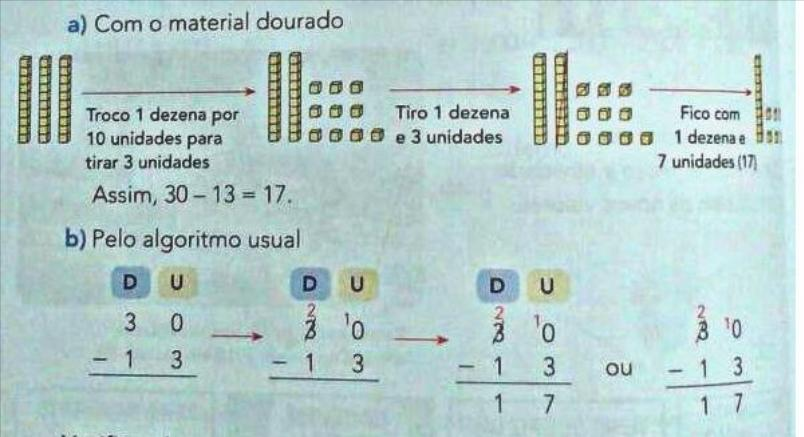
\includegraphics[width=.75\textwidth]{articles/05-material-dourado-com/figura2.jpeg}%
        \caption*{Fonte: \textcite[p.~126]{DANTE2015Projeto}.}%
        \label{fig:dante-subtracao}%
    \end{figure}%

    Assim, o “pegar emprestado” ganha significado para o aluno que passa a entender que há um desagrupamento, uma “transformação” de 1 (um) elemento em 10 (dez), de um grupo abaixo dele. Aqui se utiliza a expressão “fazer troca” ao invés de “pedir emprestado”, pois essa última sugere uma devolução. Quem pediu emprestado tem que devolver.

    \section{Relato da experiência}

    Nesta seção relata-se a experiência de intervenção realizada numa turma do 4º ano --- turno vespertino --- da Escola Estadual Isabel Oscarlina Marques, localizada no município de Santa Cruz/RN cujo objetivo era analisar as contribuições do uso do Material Dourado na compreensão do algoritmo da subtração com reserva.

    A Escola em questão atende cerca de 780 (setecentos e oitenta) alunos do Ensino Fundamental e EJA, distribuídos nos três turnos e conta com 17 (dezessete) funcionários e 30 (trinta) professores graduados na área em que atuam. A estrutura física da escola conta com 10 (dez) salas de aula, quadra esportiva (sem cobertura), secretaria, direção, auditório, sala dos professores, cozinha, refeitório, sala de multimídia, biblioteca e laboratório de informática. Também possui um acervo de materiais didáticos adequados e necessários para o desenvolvimento das aulas, como: televisão, aparelho de som, datashow, notebook, caixas amplificadas, microfones, jogos pedagógicos, entre outros.  

    Quanto aos participantes da pesquisa, foram 14 (catorze) alunos, dos quais 6 (seis) eram do sexo masculino e 8 (oito) do sexo feminino. Todos numa faixa etária entre 10 a 12 anos. 

    Inicialmente, realizou-se reunião com a direção e a coordenação da Escola com o objetivo de apresentar o tema do trabalho: O Material Dourado como recurso didático no ensino do algoritmo da subtração com reserva, bem como pedir permissão para desenvolvê-lo na supracitada instituição. Após, foi apresentada a professora do 4º ano --- vespertino ---, da turma onde seriam realizadas as atividades referentes ao trabalho de pesquisa.  Com ótima acolhida, ela falou sobre a turma nos vários aspectos do ensino-aprendizagem, principalmente no que diz respeito às dificuldades dos alunos no algoritmo da subtração, objeto da pesquisa.  

    Ao se indagar sobre o Material Dourado a professora respondeu que já havia utilizado na sala de aula, mas apenas como demonstração, não realizando nenhuma atividade em que os alunos tivessem a oportunidade de manusear o material. A partir dessas informações percebeu-se que seria viável trabalhar nesta turma o tema em estudo, mediante o perfil traçado preliminarmente pela docente a respeito dos alunos com dificuldades na aprendizagem da subtração com reserva e o fato de a professora não ter utilizado nenhum material manipulável para trabalhar tal conteúdo.  

    De acordo com \textcite{LORENZATO2006Começar}, há uma diferença pedagógica entre uma aula em que o professor apresenta o assunto ilustrando-o com material didático manipulável e uma aula em que os alunos manuseiam o material. Segundo este autor: 

    \begin{quotation}
        O material didático manipulável é o mesmo nas duas situações de ensino, mas os resultados no segundo tipo de aula “serão mais benéficos à formação dos alunos, porque, de posse do material didático manipulável, as observações e reflexões deles são mais profícuas, uma vez que poderão, em ritmos próprios, realizar suas descobertas e, mais facilmente, memorizar os resultados obtidos durante suas atividades \cite[p.~27]{LORENZATO2006Começar}. 
    \end{quotation}

    Dentre os diversos materiais didáticos manipuláveis disponíveis, optou-se pelo Material Dourado por diversos motivos. Primeiramente, porque esse material prioriza a educação sensorial da criança e destina-se a atividades que auxiliam o ensino e a aprendizagem de sistema de numeração decimal-posicional e dos métodos para efetuar as operações fundamentais. Depois, pelas características de material versátil, prático e visual que permite trabalhar a subtração com reserva de uma forma mais fácil de ser entendida e aceita, acreditando-se que: 

    \begin{quotation}
        O trabalho com os materiais concretos torna o processo de construção do sistema numérico mais acessível às crianças, pelas ações que elas realizam sobre eles --- fazer, desfazer grupos, trocar --- do que pelas representações dos elementos. Cada contexto ambiental é um marco na construção do conceito de número, que permite o gradual afastamento dos elementos concretos para a evolução na direção de um sistema mais abstrato e eficiente \cite[p.~65]{GOLBERT1999Matemática}.
    \end{quotation}

    Na verdade, o fator determinante para a escolha do Material dourado foi por ele permitir a composição e decomposição dos numerais para visualizar o processo da subtração com reserva, assim, o “pedir emprestado” passa a ter uma imagem concreta, facilitando, desse modo, a compreensão do aluno sobre o referido processo. 

    Várias são as operações possíveis de serem realizadas com esse recurso, todas elas pressupõem o entendimento anterior das representações e das regras de agrupamentos e desagrupamentos, mas neste trabalho relata-se apenas as atividades relativas à subtração com reserva que é objeto deste estudo.

    \subsection{1º encontro}

    Inicialmente, a professora fez a apresentação da turma, falando sobre o período de atividades de estágio na sala e o propósito da ação. Em seguida, realizou uma atividade de subtração que já estava prevista em seu planejamento. Ela leu um problema do livro didático e resolveu na lousa com ajuda dos alunos, indagando como deveria proceder.  

    Após, aplicou-se a atividade diagnóstica que iria orientar no planejamento de intervenção. Durante a aplicação da atividade observou-se como os alunos resolviam as questões propostas, indagando-os, com a finalidade de verificar que raciocínio eles estavam utilizando para resolver tais questões, no entanto, sem nenhuma interferência na resolução. Recomendou-se, assim, que deveriam resolver as situações-problema utilizando a operação que julgassem correta, ou necessária. Eram quatro questões que traziam problemas envolvendo a subtração com e sem reserva. Percebeu-se claramente que a maioria sentia dificuldade em operar na subtração com reserva, ou seja, quando o minuendo é menor que o subtraendo.  

    A partir dessas constatações adotou-se uma metodologia de trabalho em sala de aula utilizando o Material Dourado como recurso didático para trabalhar com o algoritmo da subtração com reserva.

    \subsection{2º encontro}

    No primeiro momento apresentou-se o Material Dourado, percebendo-se que os alunos já conheciam, pois identificaram cada peça (cubinho, barra, placa e cubo). No entanto, como eles nunca haviam manuseado esse material, reservou-se 20 minutos para brincarem à vontade com ele, fazendo-se construções livres. Pois como afirma Lorenzato:  

    \begin{quotation}
        Ao “ver com as mãos” é mais popular do que geralmente se supõe: você já viu alguém numa loja escolher roupas sem passar as mãos nelas? E crianças em loja de brinquedos conseguem apenas olhá-lo? [\dots] As pessoas precisam “pegar pra ver” como dizem as crianças \cite[p.~18]{LORENZATO2006Começar}.
    \end{quotation}

    \begin{figure}[ht]%
        \centering%
        \caption{Alunos fazendo construções livres com o Material Dourado}%
        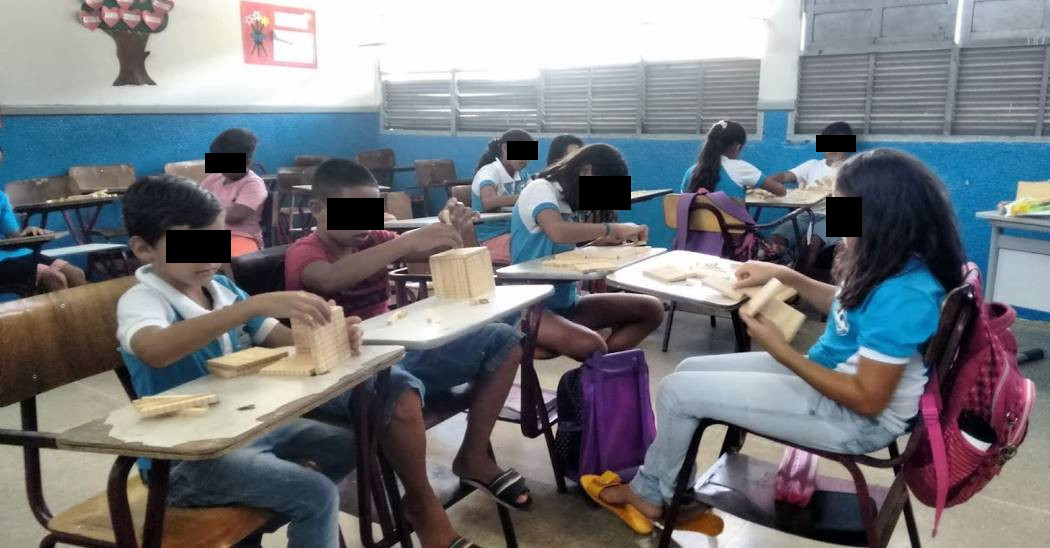
\includegraphics[width=.5\textwidth]{articles/05-material-dourado-com/figura3.jpeg}%
        \caption*{Fonte: Arquivo pessoal.}%
        \label{fig:construcoes-livres-material-dourado}%
    \end{figure}%

    Dienes \cite[apud][p.~34]{TOLEDOAndTOLEDO1997Didática} sugere que “sempre se deve iniciar a construção de um novo conceito a partir da utilização de materiais de apoio”.

    Ainda de acordo com esses autores: 

    \begin{quotation}
        Quando se oferece um material novo para as crianças, a primeira atividade que se recomenda é sempre o jogo livre: apresenta-se o material às crianças e deixa-se que elas utilizem como quiserem [\dots]. A segunda etapa é o jogo com regras, em que se propõe à criança atividades planejadas [\dots]. \cite[p.~72--73]{TOLEDOAndTOLEDO1997Didática}.
    \end{quotation}

    Após o momento de apreciação das construções livres, solicitou-se que fizessem montagens, como: uma barra feita de cubinhos; uma placa feita de barras; um cubo feito de placas, ao mesmo tempo fazendo-se perguntas onde os alunos pudessem estabelecer relações entre as peças. Por exemplo: Quantos cubinhos precisam enfileirar para formar uma barra? Quantas barras são necessárias para formar uma placa? Com quantas placas se forma um cubo?  

    O objetivo era trabalhar primeiro o Sistema de Numeração Decimal (SND), por entender que este é pré-requisito para o bom entendimento do algoritmo da subtração. O propósito era despertar a atenção dos alunos para a percepção de que o cubo é formado por 10 placas, que a placa é formada por 10 barras, e a barra é formada por 10 cubinhos. As crianças participaram ativamente da atividade e a maioria não teve dificuldade para responder os questionamentos. 

    Para finalizar, propôs-se o jogo do Nunca Dez. O objetivo desse jogo também era a compreensão do SND, ou seja, dos agrupamentos de dez em dez (dez unidades formam uma dezena, dez dezenas formam uma centena etc.), característicos do sistema decimal que possibilita fazer agrupamentos de 10 em 10, assim como fazer reagrupamentos, fazer trocas, estimulando o cálculo mental.  

    Para essa atividade formou-se um grande grupo. Cada criança, na sua vez de jogar, lançava o dado e retirava para si a quantidade de cubinhos correspondente à soma dos dois dados. O número que sobressaía no dado dava direito a retirar somente cubinhos. Toda vez que uma criança juntava 10 cubinhos, ela deveria trocar os 10 cubinhos por uma barra. Da mesma maneira, quando tivesse 10 barrinhas poderia trocá-las por uma placa. Previamente foi combinado que o jogo terminaria quando algum aluno conseguisse formar duas placas. 

    \begin{figure}[ht]%
        \centering%
        \caption{Alunos jogando ``Nunca Dez''}%
        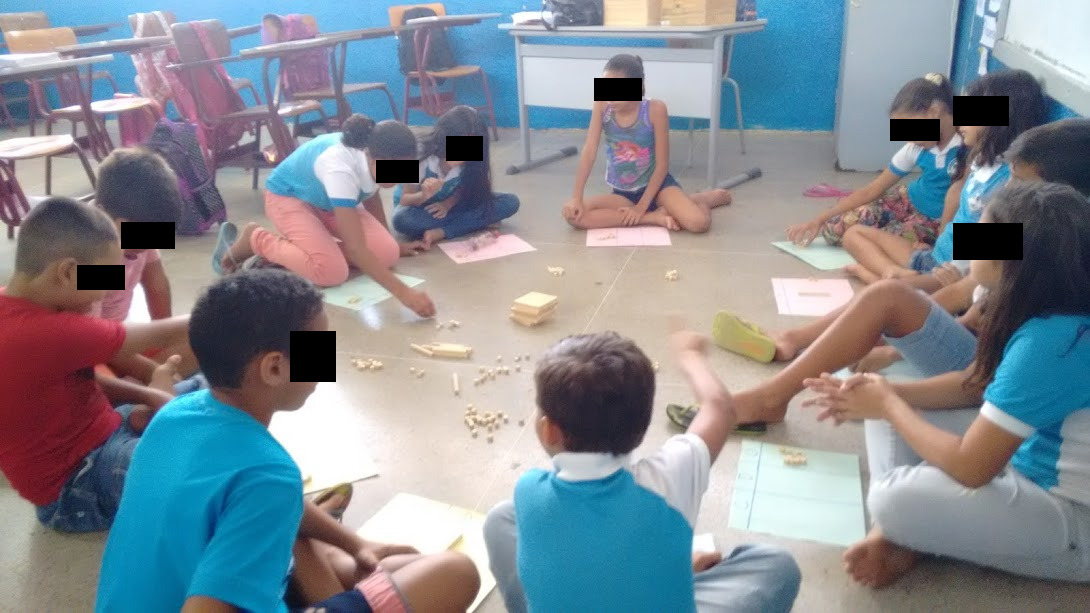
\includegraphics[width=.5\textwidth]{articles/05-material-dourado-com/figura4.jpeg}%
        \caption*{Fonte: Arquivo pessoal.}%
        \label{fig:nunca-dez}%
    \end{figure}%

    Na primeira rodada do jogo, alguns alunos sentiram dificuldade em perceber quando deveriam fazer as trocas, precisando de orientação, mas logo entenderam a dinâmica, e o jogo fluiu satisfatoriamente, constatando-se que a maioria ia fazendo as trocas necessárias. O mais interessante era que ficavam fiscalizando as trocas dos seus colegas. Apenas um aluno precisou de ajuda durante mais tempo. Assim, verificou-se que o Material Dourado facilitou a compreensão do “pedir emprestado” que foi substituído por “fazer trocas”.  

    Centurión afirma que:  

    \begin{quotation}
        Para que os desagrupamentos e trocas possam ser feitos e entendidos pelo aluno no algoritmo da subtração com reserva, é preciso que este aluno tenha compreendido muito bem nosso sistema de numeração posicional de base dez, no qual um algarismo à esquerda de outro vale dez vezes mais do que valeria se ocupasse aquele lugar. É isto que nos permite desagrupar uma centena e transformá-la em dez dezenas; desagrupar uma dezena e trans\-for\-má-la em dez unidades \cite[p.~186]{CENTURIÓN1995Números}.
    \end{quotation}

    Nessa perspectiva, realizou-se um trabalho voltado para o SND, acreditando-se que quando os alunos já conhecem as características da escrita numérica e já estão familiarizados com agrupamentos e trocas na base 10, é possível desenvolver a técnica operatória da subtração com reserva de modo lógico e, portanto, compreensivo.

    \subsection{3º encontro}

    Iniciou-se com a realização de uma atividade denominada “Quanto vou ficar”. Cada aluno após sortear uma ficha teria que representar o número nela contido e, em seguida, realizar a operação de subtração com reserva impressa no verso da ficha, com o auxílio do Material Dourado. O objetivo era perceber as possíveis dificuldades que alguns alunos apresentavam e intervir diretamente a fim de superá-las.  

    Ao final, pediu-se que comentassem o que acharam da atividade. Um aluno falou, entusiasmado: \textit{--- agora compreendo por que estou fazendo as trocas}. Outro respondeu que \textit{``com essas peças fica mais fácil entender por que o 3 virou 13''}.

    \begin{figure}[ht]%
        \centering%
        \caption{Realizando a atividade denominada ``Quanto vou ficar?''}%
        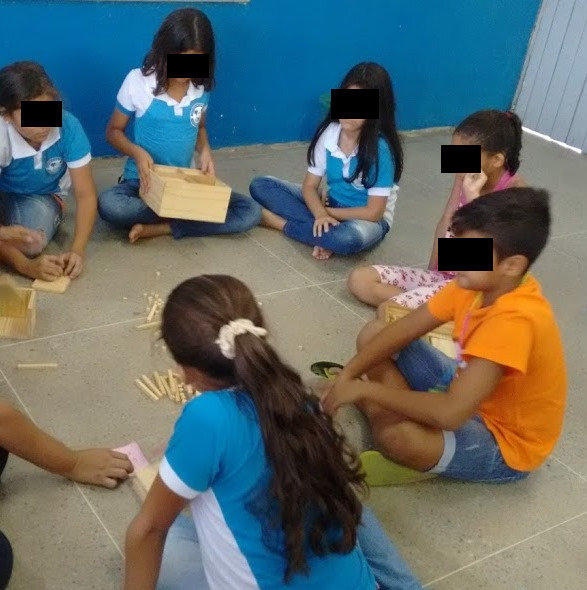
\includegraphics[width=.5\textwidth]{articles/05-material-dourado-com/figura5.jpeg}%
        \caption*{Fonte: Arquivo pessoal.}%
        \label{fig:quanto-vou-ficar}%
    \end{figure}%

    Com essas atividades foi possível perceber que os alunos ao fazerem cálculos com o auxílio do Material Dourado, assimilaram melhor os conceitos básicos presentes na técnica operatória da subtração, como também interagiram com os colegas, trocando ideias e argumentando quando seus resultados divergiam do colega. Assim, consideraram que aprenderam Matemática de forma divertida e prazerosa. 

    Dando continuidade à aula realizou-se uma atividade de subtração xerografada (copiada). Os alunos foram orientados de que deveriam primeiro representar o minuendo com o Material Dourado, em seguida realizar a subtração, e só depois  iriam  anotar  o resultado. À medida que iam realizando as operações os alunos foram solicitados a falar sobre os procedimentos utilizados por eles, sendo mediados nas representações escritas.  

    Percebeu-se que alguns aprenderam mais rapidamente e outros apresentavam algumas dificuldades. Entretanto, foram notórias a concentração dos alunos durante a atividade e a satisfação em estar manuseando o material. Pegavam com muita atenção, tinham cuidado para não perder as peças e quando estavam representando os dados das situações refletiam (trocavam ideias) a cada momento, fixando os olhares nas peças e analisando como realizariam a operação.  

    Desse modo, pode-se concluir que essas atividades favoreceram as crianças a criarem suas próprias estratégias, gerando confiança e autonomia. Assim, diante das peças e utilizando o processo de contagem, realizaram a operação de subtração corretamente, pois podiam ver as barrinhas das dezenas contidas na placa da centena e os cubinhos referentes às unidades, ou melhor, podiam representar com as peças as situações propostas, e mais que isso, visualizar as trocas com material concreto, o que indubitavelmente facilitou a compreensão do processo envolvido na operação.

    \begin{figure}[ht]%
        \centering%
        \caption{Momento da atividade}%
        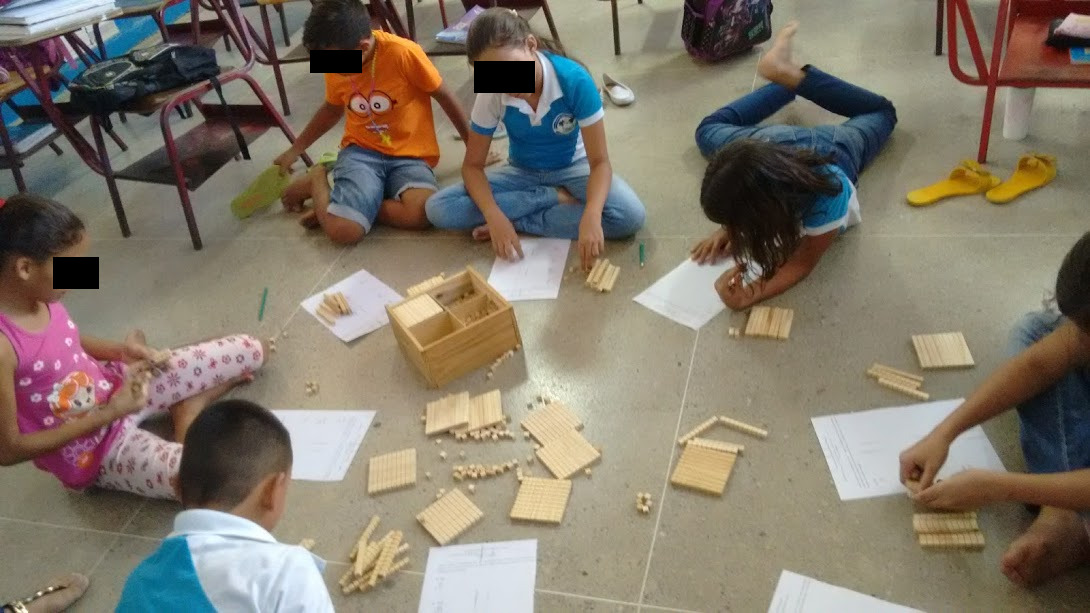
\includegraphics[width=.5\textwidth]{articles/05-material-dourado-com/figura6.jpeg}%
        \caption*{Fonte: Arquivo pessoal.}%
        \label{fig:momento-atividade}%
    \end{figure}%

    \subsection{4º encontro}

    Finalizando os encontros, procederam-se duas atividades: uma individual, trabalhando o algoritmo da subtração com o Material Dourado impresso, a outra, do livro didático do aluno. Em relação à primeira, eles teriam que efetuar “as trocas” através de desenhos. Durante o desenvolvimento dessa atividade observou-se que o Material Dourado ajudou a superar a ideia de que na subtração “pede-se emprestado”, ou seja, o aluno percebeu que, na verdade, não se pede emprestado e sim, realizam-se trocas. O que se faz é decompor uma centena e acrescentar às dezenas, ou decompor uma dezena e acrescentar às unidades, enfim, deve-se entender que há um desagrupamento, uma “transformação” de 1 (um) elemento em 10 (dez) de um grupo de menor valor que ele. 

    \begin{figure}[ht]%
        \centering%
        \caption{Aluna realizando a atividade com material dourado através de desenho}%
        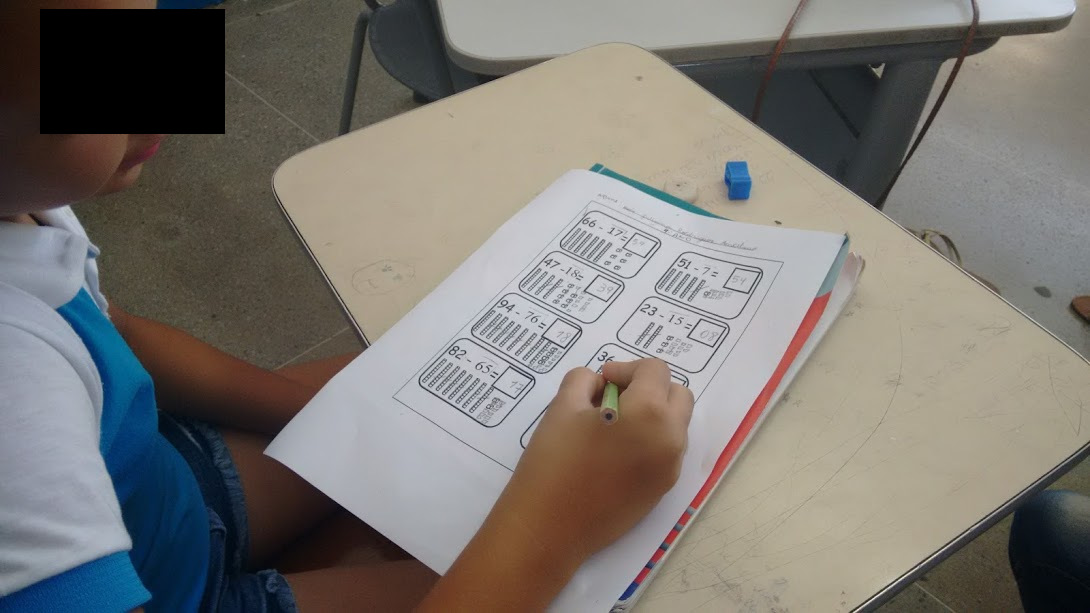
\includegraphics[width=.5\textwidth]{articles/05-material-dourado-com/figura7.jpeg}%
        \caption*{Fonte: Arquivo pessoal.}%
        \label{fig:md-desenho}%
    \end{figure}%

    No que se refere à atividade do livro didático a intenção era verificar se os alunos conseguiam resolver as subtrações com reserva propostas no seu livro. Observou-se que a maioria conseguiu realizar sem auxílio, o que possibilitou concluir que o Material Dourado foi um recurso facilitador nesse processo, pois ajudou aos alunos compreenderem melhor os conteúdos matemáticos trabalhados, propiciando também a interação e a troca de saberes, de maneira que eles tiveram a oportunidade de desenvolver e socializar seus conhecimentos. Sem dúvida, esse material despertou a atenção e o interesse dos alunos envolvidos nesta pesquisa, favorecendo ainda a concentração, além de permitir o contato com o concreto para depois realizar as abstrações pertinentes ao algoritmo da subtração.

    \section{Considerações finais}

    Neste artigo relata-se uma experiência com a utilização do Material Dourado como recurso didático para auxiliar na compreensão do SND e na aprendizagem do algoritmo da subtração com reserva numa turma do 4º ano do Ensino Fundamental. Com essa intervenção, foi possível perceber a evolução cognitiva das crianças envolvidas na pesquisa com relação à aprendizagem da subtração com reserva, pois à medida que se realizavam os trabalhos notava-se, gradativamente, que as dificuldades iam sendo superadas e que aumentava o interesse da turma para realizar as atividades propostas.  

    Essa experiência possibilitou compreender a importância de se trabalhar com metodologias que favorecem aos alunos refletirem sobre as ações realizadas e assim possam construir um saber significativo, desenvolvendo habilidades que lhes permitam passar mais facilmente do concreto para o abstrato. Nessa concepção, propôs-se através do Material Dourado construir o conceito de subtração a partir do concreto, ou seja, o aluno constrói o seu conhecimento, adquirindo base para a abstração; favorecer o questionamento quanto à construção dos conceitos; e quebrar a rotina da aula, propiciando uma maior socialização, interação e interesse da turma.  

    Assim, a aprendizagem se torna mais interessante, pois a partir dessas atividades diferenciadas estimula-se a atenção dos educandos e promove-se também sua autoconfiança. Além disso, a manipulação do concreto faz com que os alunos se sintam agentes de seu próprio conhecimento, uma vez que criam seus métodos e não seguem procedimentos mecânicos e vazios de significado, isto é, sem compreenderem o que estão fazendo. 

    É importante ressaltar que o uso do Material Dourado com o intuito de tornar a aula diferente, alegre, utilizando-o apenas como um recurso motivador, não é suficiente, pois é preciso planejar, definir os objetivos, acreditar que não é uma simples brincadeira, mas sim uma ferramenta importante para um processo de ensino e aprendizagem com qualidade. É fundamental que, paralelamente ao desenvolvimento de atividades, o fazer pedagógico favoreça o pensar matemático, ou seja, os alunos possam reconhecer os conteúdos abordados nas atividades presentes do dia a dia, fazendo as possíveis relações e descobrindo as regularidades existentes.  

    Assim, torna-se imprescindível que a escola implemente projetos visando à melhoria do processo ensino-aprendizagem por meio de ações que priorizem o desenvolvimento integral do aluno e a participação efetiva de todos os envolvidos no processo. Isso só acontecerá se houver uma mudança de atitude, um repensar da prática do professor em prol de uma metodologia que favoreça aos alunos a construção de novos conceitos, sempre apoiados em conceitos já existentes na sua estrutura cognitiva.  

    Dessa forma, conclui-se que o uso do Material Dourado atende a essas expectativas, pois possibilita aos alunos refletirem sobre as ações realizadas, permitindo a construção de um saber significativo com o desenvolvimento de habilidades que propiciam a abstração das construções realizadas, transformando-as em conhecimentos adquiridos efetivamente, atingindo assim o objetivo dessa pesquisa.  

    As experiências no Curso de Especialização em Matemática proporcionaram suportes que subsidiaram na relação entre teoria e prática, apontando os caminhos para que essa pesquisa se desenvolvesse satisfatoriamente. Essa investigação evidencia a necessidade de se trabalhar com metodologias diferenciadas em que os alunos são participantes diretos na construção e significação do conhecimento, bem como destaca a importância da formação continuada do professor para superar as dificuldades que permeiam o ensino de Matemática. Assim, ao término deste trabalho, pode-se afirmar que o uso do Material Dourado no ensino da Matemática, além de facilitar a compreensão do desagrupamento na subtração, dá às relações numéricas abstratas uma imagem mais concreta, facilitando a compreensão e o desenvolvimento do raciocínio lógico, tornando o aprendizado bem mais agradável, pois é dada ao aluno a oportunidade de construir seus conhecimentos de uma forma mais interativa, dinâmica e prazerosa.   

    Conclui-se, então, que a metodologia utilizada nesse trabalho atendeu a expectativa da pesquisadora, atingindo assim o objetivo proposto. Por isso, pode ser utilizada pelos docentes que acreditam numa educação eficaz e prazerosa, capaz de motivar o estudante em prol do seu conhecimento. 

    \nocite{NETO2005Didática}
    \nocite{PANNIZA2006Ensinar}

    \printbibliography[heading=subbibliography,notcategory=fullcited]

    \label{chap:material-douradoend}

\end{refsection}
